\documentclass[11pt]{exam}

%---enable russian----

\usepackage[utf8]{inputenc}
\usepackage[russian]{babel}



\usepackage[margin=0.73in]{geometry}
%\usepackage[top=1in, bottom=1in, left=1in, right=1in]{geometry}

\usepackage{graphicx}
\usepackage{url}
\usepackage{latexsym}
\usepackage{amscd,amsmath,amsthm}
\usepackage{mathtools}
\usepackage{amsfonts}
\usepackage{amssymb}
\usepackage[dvipsnames]{xcolor}
\usepackage{hyperref}

\usepackage{algorithmicx, enumitem, algpseudocode, algorithm, caption}
\usepackage{tikz}
\usetikzlibrary{arrows,decorations.pathmorphing,backgrounds,calc}
\usetikzlibrary{chains, matrix, positioning, scopes, patterns, shapes}
\usepackage{pgfplots, subfigure}
\usetikzlibrary{automata}

%%%%%%%%%%%%%%%%%%%%%
% Handling comments and versions %%%
%%%%%%%%%%%%%%%%%%%%%

%\renewcommand{\comment}[1]{\texttt{[#1]}}


%%%%%%%%%%%%%%%%%%%%%%%%%%%
%% THEOREMS
%%%%%%%%%%%%%%%%%%%%%%%%%%%

\newtheorem{theorem}{Theorem}[section]
\newtheorem{axiom}[theorem]{Axiom}
\newtheorem{conclusion}[theorem]{Conclusion}
\newtheorem{condition}[theorem]{Condition}
\newtheorem{conjecture}[theorem]{Conjecture}
\newtheorem{corollary}[theorem]{Corollary}
\newtheorem{criterion}[theorem]{Criterion}
\newtheorem{definition}[theorem]{Definition}
\newtheorem{lemma}[theorem]{Lemma}
\newtheorem{notation}[theorem]{Notation}
\newtheorem{proposition}[theorem]{Proposition}


\theoremstyle{definition}
\newtheorem{problem}{Problem}


\newcommand{\nc}{\newcommand}
\nc{\eps}{\varepsilon}
\nc{\RR}{{{\mathbb R}}}
\nc{\CC}{{{\mathbb C}}}
\nc{\FF}{{{\mathbb F}}}
\nc{\NN}{{{\mathbb N}}}
\nc{\ZZ}{{{\mathbb Z}}}
\nc{\PP}{{{\mathbb P}}}
\nc{\QQ}{{{\mathbb Q}}}
\nc{\UU}{{{\mathbb U}}}
\nc{\OO}{{{\mathbb O}}}
\nc{\EE}{{{\mathbb E}}}

\newcommand{\val}{\operatorname{val}}
\newcommand{\wt}{\ensuremath{\mathit{wt}}}
\newcommand{\Id}{\ensuremath{I}}
\newcommand{\transpose}{\mkern0.7mu^{\mathsf{ t}}}
\newcommand*{\ScProd}[2]{\ensuremath{\langle#1\mathbin{,}#2\rangle}} %Scalar Product
\renewcommand{\char}{\ensuremath{\mathsf{char}}}

\DeclareMathOperator{\Vol}{Vol}

%\pretolerance=1000

%%%%%%%%%%%%%%%%%%%%%%%%%%%%%%%%
%%%%%%%%%%%%%%%%%%%%%%%%%%%%%%%%
%% DOCUMENT STARTS
%%%%%%%%%%%%%%%%%%%%%%%%%%%%%%%%
%%%%%%%%%%%%%%%%%%%%%%%%%%%%%%%%


\begin{document}	
	{\noindent
		\textsc{БФУ им. И. Канта -- Компьютерный практикум по криптографии на эллиптических кривых }\\[5pt]
		Преподаватель {С. Новоселов}   \hfill{Осень 2025\\}
	\hrule
	\begin{center}
		{\LARGE\textbf{
				Лекция 1. Введение \\[5pt]
		}}
		
	\end{center}
	\hrule \vspace{5mm}
	
	\thispagestyle{empty}
	
	Эллиптические кривые используются в криптографии как основа для построения множества криптографических примитивов, схем и протоколов, таких как цифровых подписи и схемы обмена ключами.
	
	В настоящее время в криптографии выделяется два направления: классическая криптография и посквантовая. К классической криптографии относятся криптографические схемы, построенные на основе сложности задач дискретного логарифмирования, факторизации целых чисел и других. Однако, данные задачи могут быть взломаны на квантовом компьютере за полиномиальное время. В связи с этим появилось новое направление криптографических исследований -- постквантовая криптография требует от схем стойкость к атакам на квантовом компьютере.
	
	Среди распространённых классических схем на эллиптических кривых имеются схема подписи (ECDSA) и обмен ключами по протоколу Диффи-Хэлмана на эллиптических кривых (ECDH).
	
	Из перспективных постквантновых схем на эллиптических кривых можно отметить схемы, построенные на сложности задачи вычисления изогении между эллиптическими кривыми --  цифровую подпись SQISign и схему обмена ключами CSIDH.
	
	Классическая криптография в настоящее время широко используется на практике в большом числе приложений.
	
	\begin{enumerate}
		\item Обмен ключами и цифровые подписи в протоколе HTTPS (TLS), который используется для шифрования данных при доступе к ресурсам в интернете (см. Рис.~\ref{fig:tls:example}).
		\item В составе протоколов для построения VPN: обмен ключами в протоколе WireGuard, встроенном в ядро Linux, осуществляется на базе эллиптической кривой Curve25519.
		\item Кривые Эдвардса Ed25519 можно использовать для цифровой подписи в протоколе SSH.
		\item Bitcoin/Ethereum используют кривую Secp256k1 для цифровой
		подписи транзакций.
	\end{enumerate}

	\begin{figure}
		\caption{Пример. Wikipedia использует сертификат на основе ECDSA}
		\label{fig:tls:example}
		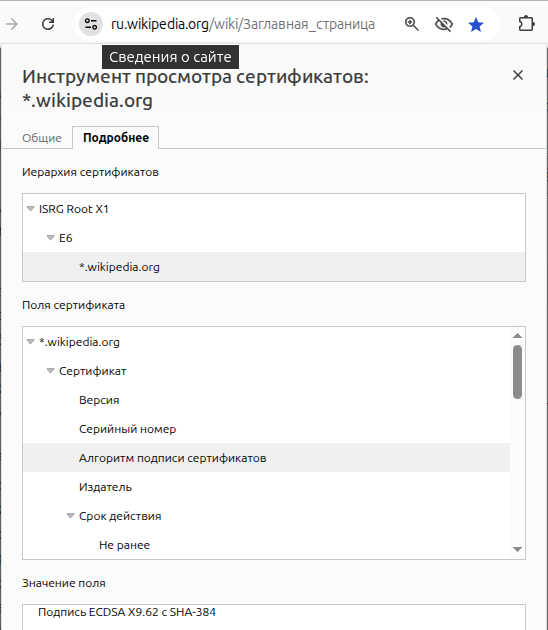
\includegraphics[scale=0.5]{../images/example_tls}
	\end{figure}
	
	Хотя на практике современные квантовые компьютеры в настоящее время не могут взломать классические криптосистемы на эллиптических кривых, предполагается, что такие компьютеры могут быть созданы в течении 10 лет.
	
	Полный отказ от классической криптографии (ECDSA,
	ECDH, FFDH, RSA) рекомендован NIST начиная с 2035 года. А с 2030 года классические схемы объявлены устаревшими. Это значит, что начиная с этих дат будет прекращена поддержка классической криптографии в популярных протоколах сети Интернет (TLS, https, ssh).
	
	В качестве замены предлагаются различные схемы постквантовой криптографии. В эллиптической криптографии, это SQISign вместо ECDSA, CSIDH вместо ECDH. Однако, в настоящее время схемы на изогениях не утверждены в качестве стандартов.
	
\section{План курса}
\begin{enumerate}
	\item Введение
	\item Групповой закон на эллиптической кривой
	\item Точки $n$-кручения
	\item Алгоритмы подсчета $\mathbb{F}_q$-рациональных точек кривой
	\item Алгоритм факторизации на эллиптических кривых
	\item Тест на простоту Goldwasser-Kilian
	\item Выбор эллиптической кривой для криптографии
	\item Криптографические схемы на изогениях
\end{enumerate}

Заметим, что и классическая криптография и постквантовая криптография имеют одну и ту же теоретическую базу. И всё, что используется в классической криптографии на эллиптических кривых, используется и в посткватновой. Поэтому мы начинаем с классической криптографии и потом переходим к постквантовой.

\section{Порядок работы}
Формат: лекции + сдача лабораторных работ.
\vspace{0.5em}
\begin{itemize}
	\item после лекций выкладываются лабораторные работы
	\item срок сдачи: {2} недели
	\item за пределами срока сдачи работы принимаются с низким приоритетом и в количестве не более {2} за пару
\end{itemize}
\vspace{0.5em}
{Экзамен}: сдать {85\%} лабораторных и {курсовую}.
\begin{itemize}
	\item оценка -- среднее по оценкам за сдачу лабораторных
\end{itemize}

\section{Основные определения}
	Уравнение Вейерштрасса \textbf{в аффинных координатах}:
\begin{equation}\label{eq:weierstrassequation}
	f: y^2+a_1xy + a_3y = x^3 + a_2x^2 + a_4x + a_6
\end{equation}

Уравнение над полем~$K$ -- \textbf{гладкое}, если во множестве его решений над~$\overline{K}$ нет сингулярных точек.
\vspace{1em}

\textbf{Эллиптическая кривая} задаётся как \[E(K) = \{ (x,y) \in K \times K: f(x,y)=0 \} \cup \{\mathcal{O}\}
\]
для гладкого~$f$.
\begin{itemize}
	\item $\mathcal{O}$ -- точка в бесконечности.
	\item $K$ -- некоторое поле, чаще всего $K = \mathbb{F}_q$.
\end{itemize}

\textbf{Уравнение Вейерштрасса} в проективных координатах: 
\begin{equation}
	\label{eq:weierstrass}
	F: Y^2Z + a_1 X Y Z + a_3 Y Z^2 = X^3 + a_2 X^2 Z + a_4 X Z^2 + a_6 Z^3,
\end{equation}
где $a_i \in K$.
\begin{itemize}
	%\item \structure{гладкое} (или несингулярное): $\forall P \in \mathbb{P}^2(K)$, $\frac{dF}{dX}(P) \neq 0$, $\frac{dF}{dY}(P) \neq 0$ или $\frac{dF}{dZ}(P) \neq 0$.
	\item \textbf{сингулярное}: $\exists P \in \mathbb{P}^2(K): \frac{dF}{dX}(P) = \frac{dF}{dY}(P) = \frac{dF}{dZ}(P) = 0$.
	\item  \textbf{гладкое} (или несингулярное) в противном случае.
\end{itemize}
%\footnotetext[1]{проективная плоскость над $K$ — множество классов эквивалентности на $K^3\setminus \{0,0,0\}$, т.е. $\overrightarrow{X} \sim \overrightarrow{Y}$, если $x_1=u*y_1,x_2=u*y_2,x_3=u*y_3$ }
%\structure{Эллиптическая кривая}:

\vspace{1em}

\textbf{Эллиптическая кривая $E$} -- множество точек $\mathbb{P}^2(K)$, удовлетворяющих гладкой кривой \eqref{eq:weierstrass}.

\begin{itemize}
	\item Точка в бесконечности: $\exists! \mathcal{O} = (0: 1: 0)$.
\end{itemize}

\begin{itemize}
	\item Проективные координаты позволяют избежать деления в арифметике за счёт доп. умножений.
\end{itemize}

\subsection{Дискриминант}
Как проверить, что уравнение Вейерштрасса задаёт эллиптическую кривую? Для решения задачи используется дискриминант кривой. Обозначим
\begin{equation}
	\begin{split}
		d_2 &= a_1^2 + 4a_2 \\
		d_4 &= 2a_4 + a_1a_3 \\
		d_6 &= a_3^2 + 4a_6 \\
		d_8 &= a_1^2a_6 + 4a_2a_6 - a_1a_3a_4 + a_2a_3^2 - a_4^2 \\
		c_4 &= d_2^2 - 24d_4 \\
		%\text{Для проверки: } 4d_8 &= d_2d_6 - d_4^2
	\end{split}
\end{equation}
Тогда \textbf{дискриминант} уравнения \eqref{eq:weierstrassequation} определяется как 
\[
\Delta = -d_2^2d_8 - 8d_4^3-27d_6^2+9d_2d_4d_6.
\]

\begin{theorem}[Silverman, Th.~1.4]
~
\begin{enumerate}
	\item $\Delta \neq 0 \iff$ кривая гладкая ($\implies$ задаёт эллиптическую кривую) 
	\item $\Delta = 0, c_4 \neq 0 \iff$ кривая обладает узлом (node) 
	\item $\Delta = c_4 = 0 \iff$ кривая обладает точкой перегиба (cusp)
\end{enumerate}
\end{theorem}

	\begin{figure}[h!]
		\caption{Случай $\Delta < 0$}
		\begin{tikzpicture}
			\begin{axis}[
				xmin=-5,
				xmax=5,
				ymin=-7,
				ymax=7,
				xlabel={$x$},
				ylabel={$y$},
				scale only axis,
				axis lines=middle,
				domain=-2.1038:3,
				samples=200,
				smooth,
				clip=false,
				axis equal image=true,
				]
				\addplot [red] {sqrt(x^3-3*x+3)}
				node[right] {$y^2=x^3-3x+3$};
				\addplot [red] {-sqrt(x^3-3*x+3)};
			\end{axis}
		\end{tikzpicture} 
	\end{figure}

	\begin{figure}[h!]
			\caption{Случай $\Delta > 0$}
			\centering
			\begin{tikzpicture}
				\begin{axis}[
					xmin=-1.5,
					xmax=1.5,
					ymin=-2,
					ymax=2,
					xlabel={$x$},
					ylabel={$y$},
					scale only axis,
					axis lines=middle,
					domain=-1:0, 
					samples=200,
					smooth,
					clip=false,
					axis equal image=true,
					]
					\addplot [red] {sqrt(x^3-x)};
					\addplot [red] {-sqrt(x^3-x)};
				\end{axis}
				\begin{axis}[
					xmin=-1.5,
					xmax=1.5,
					ymin=-2,
					ymax=2,
					xlabel={$x$},
					ylabel={$y$},
					scale only axis,
					axis lines=middle,
					domain=0.1:1.5, 
					samples=200,
					smooth,
					clip=false,
					axis equal image=true,
					]
					\addplot [red] {sqrt(x^3-x)}
					node[right] {$y^2=x^3-x$};
					\addplot [red] {-sqrt(x^3-x)};
				\end{axis}
			\end{tikzpicture}
		\end{figure}

\subsection{Изоморфизмы эллиптических кривых}
Пусть $E_1/K, E_2/K$ -- эллиптические кривые с уравнениями:
\begin{equation}
	\begin{split}
		E_1&: y^2+a_1xy + a_3y = x^3 + a_2x^2 + a_4x + a_6 \\
		E_2&: y^2+a_1'xy + a_3'y = x^3 + a_2'x^2 + a_4'x + a_6'
	\end{split}
\end{equation}

$E_1/K, E_2/K$ \textbf{изоморфны}, если они изоморфны как проективные многообразия, т.е. $\exists$ морфизмы $\phi: E_1/K \to E_2/K, \psi: E_2/K \to E_1/K$ (определённые над $K$), такие что $\psi \circ \phi = id_{E_1}, \phi \circ \psi = id_{E_2}$.

%\begin{tcolorbox}[colframe=title-and-section-color!120, colback=title-and-section-color!5, title=Теорема, center title]
\begin{theorem}
	$E_1 \simeq E_2 \iff \exists u,r,s,t \in K, u \neq 0$ такие, что замена
\begin{equation}
	\label{eq:isom}
	(x,y) \mapsto (u^2x+r, u^3y+ u^2sx+t)
\end{equation}
преобразует кривую $E_1$ в $E_2$.
\end{theorem}
%\end{tcolorbox}

Изоморфизм кривых задаёт отношение эквивалентности.

Зачем нужны изоморфизмы на практике? Они позволяют подбирать форму кривой под нужные свойства в арифметике. Например:
\begin{itemize}
	\item с меньшим количеством коэффициентов: ускорение вычислений;
	\item с константным временем выполнения группового закона: противодействие атакам по побочным каналам.
\end{itemize}

\subsection{Краткие формы}
    \begin{equation*}
	E/K: y^2 + a_1 xy + a_3 y = x^3 + a_2 x^2 + a_4 x + a_6 \tag{\ref{eq:weierstrassequation}}
\end{equation*}
\textbf{$\operatorname{char} K \neq 2$:}
Изоморфизм \[(x, y)\mapsto \left(x, \frac{1}{2}(y-a_1x-a_3)\right)\] преобразует $E/K$ к виду:
\begin{equation}
	\label{eq:char_neq2}
	E/K: y^2 = 4x^3 + d_2x^2 + 2d_4 + d_6.
\end{equation}

\textbf{$\operatorname{char} K \neq 2, 3$:}
Изоморфизм
\[
(x, y) \mapsto \left(\frac{x-3d_2}{36}, \frac{y}{216}\right)
\]
Преобразует~\eqref{eq:char_neq2} к виду:
\begin{align}
	E/K: y^2 = x^3 + ax + b
\end{align}
\[
a = -27 c_4
\]
\[
b = -56(d_2^3 + 36 d_2 d_4 - 216 d_6) 
\]

В последнем случае, 
\begin{align*}
	\Delta &= -16(4a^3 + 27b^2) \\ \nonumber
\end{align*}
\textbf{$char K = 2$:} 
\[
a_1 \neq 0 \implies (x, y) \mapsto \left(a_1^2x+\frac{a_3}{a_1}; \, a_1^3y + \frac{a_1^2a_4+a_3^2}{a_1^3}\right)
\]
\begin{equation}
	E/K: y^2+xy=x^3+a_2'x^2+a_6'
\end{equation}

\[
a_1 \neq 0 \implies (x, y) \mapsto (x+a_2, y)
\]
\begin{equation}
	E/K: y^2+a_3y = x^3+a_4x+a_6
\end{equation}

\subsection{Определение изоморфности кривых}
\textbf{$j$-инвариант} эллиптической кривой $E$:
\[
j(E) = \frac{c_4^3}{\Delta}
\] или для краткой формы  $j(E) = -1728 \frac{4a^3}{\Delta}$.
\begin{center}
%	\begin{tcolorbox}[enhanced,hbox,colback=title-and-section-color!5,colframe=title-and-section-color!120,title=Теорема,center title]
\begin{theorem}
	$E_1 \simeq E_2$ над $\overline{K} \iff j(E_1)=j(E_2)$.
\end{theorem}
%	\end{tcolorbox}	
\end{center}
Определение изоморфности кривых над полем $K$: проверка условий теоремы. Если выполняется -- составление и решение системы уравнений используя \eqref{eq:isom}.

\subsection{Литература}
	\begin{enumerate}
		\item Washington L.C. "Elliptic curves number theory and cryptography"%. 2ed (2008)
		\item Menezes A. "Elliptic curve public key cryptosystems"
		\item Hankerson D., Menezes A., Vanstone S. "Guide to elliptic curve cryptography"
		\item Blake I., Seroussi G., Smart N. "Elliptic Curves in Cryptography"
		\item Silverman J.H. "The Arithmetic of Elliptic Curves"%, 2ed (2009)
	\end{enumerate}

\end{document}
